\documentclass[14pt]{extbook}
\usepackage{multicol, enumerate, enumitem, hyperref, color, soul, setspace, parskip, fancyhdr} %General Packages
\usepackage{amssymb, amsthm, amsmath, latexsym, units, mathtools} %Math Packages
\everymath{\displaystyle} %All math in Display Style
% Packages with additional options
\usepackage[headsep=0.5cm,headheight=12pt, left=1 in,right= 1 in,top= 1 in,bottom= 1 in]{geometry}
\usepackage[usenames,dvipsnames]{xcolor}
\usepackage{dashrule}  % Package to use the command below to create lines between items
\newcommand{\litem}[1]{\item#1\hspace*{-1cm}\rule{\textwidth}{0.4pt}}
\pagestyle{fancy}
\lhead{Progress Quiz 7}
\chead{}
\rhead{Version B}
\lfoot{4173-5738}
\cfoot{}
\rfoot{Spring 2021}
\begin{document}

\begin{enumerate}
\litem{
Choose the equation of the function graphed below.
\begin{center}
    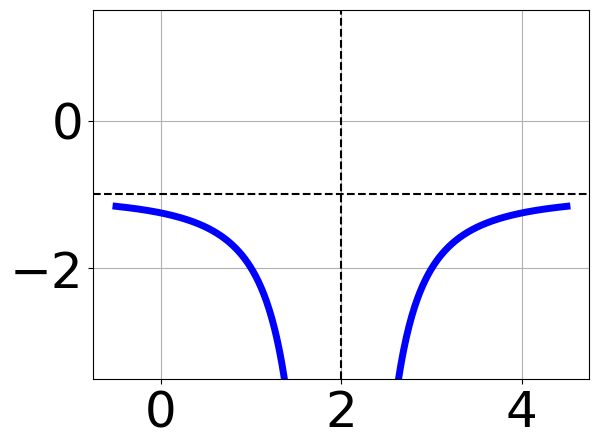
\includegraphics[width=0.5\textwidth]{../Figures/rationalGraphToEquationB.png}
\end{center}
\begin{enumerate}[label=\Alph*.]
\item \( f(x) = \frac{1}{(x + 2)^2} - 1 \)
\item \( f(x) = \frac{1}{x + 2} - 1 \)
\item \( f(x) = \frac{-1}{(x - 2)^2} - 1 \)
\item \( f(x) = \frac{-1}{x - 2} - 1 \)
\item \( \text{None of the above} \)

\end{enumerate} }
\litem{
Determine the domain of the function below.\[ f(x) = \frac{6}{18x^{2} -33 x + 15} \]\begin{enumerate}[label=\Alph*.]
\item \( \text{All Real numbers except } x = a, \text{ where } a \in [8.96, 9.38] \)
\item \( \text{All Real numbers except } x = a \text{ and } x = b, \text{ where } a \in [0.55, 0.95] \text{ and } b \in [0.97, 1.34] \)
\item \( \text{All Real numbers except } x = a, \text{ where } a \in [0.55, 0.95] \)
\item \( \text{All Real numbers except } x = a \text{ and } x = b, \text{ where } a \in [8.96, 9.38] \text{ and } b \in [29.96, 30.21] \)
\item \( \text{All Real numbers.} \)

\end{enumerate} }
\litem{
Solve the rational equation below. Then, choose the interval(s) that the solution(s) belongs to.\[ \frac{-6x}{-3x + 3} + \frac{-3x^{2}}{-18x^{2} -3 x + 21} = \frac{-3}{6x + 7} \]\begin{enumerate}[label=\Alph*.]
\item \( \text{All solutions lead to invalid or complex values in the equation.} \)
\item \( x \in [-1.17,-0.67] \)
\item \( x \in [-1.48,-1.27] \)
\item \( x_1 \in [0.08, 0.17] \text{ and } x_2 \in [-5.1,-1.4] \)
\item \( x_1 \in [0.08, 0.17] \text{ and } x_2 \in [-0.9,3.5] \)

\end{enumerate} }
\litem{
Determine the domain of the function below.\[ f(x) = \frac{3}{18x^{2} +45 x + 18} \]\begin{enumerate}[label=\Alph*.]
\item \( \text{All Real numbers except } x = a \text{ and } x = b, \text{ where } a \in [-19, -14] \text{ and } b \in [-19, -14] \)
\item \( \text{All Real numbers except } x = a, \text{ where } a \in [-2, -1] \)
\item \( \text{All Real numbers except } x = a, \text{ where } a \in [-19, -14] \)
\item \( \text{All Real numbers except } x = a \text{ and } x = b, \text{ where } a \in [-2, -1] \text{ and } b \in [-1.5, 5.5] \)
\item \( \text{All Real numbers.} \)

\end{enumerate} }
\litem{
Choose the graph of the equation below.\[ f(x) = \frac{-1}{x - 3} - 3 \]\begin{enumerate}[label=\Alph*.]
\begin{multicols}{2}\item 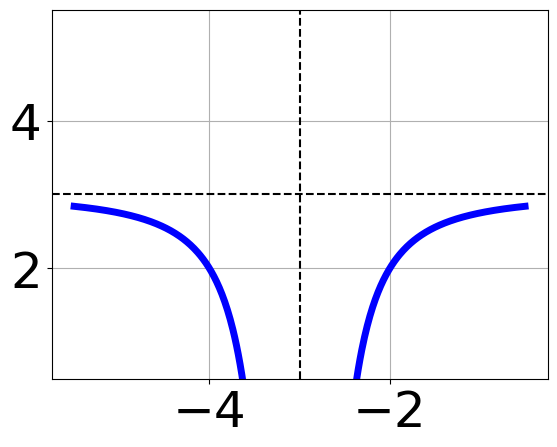
\includegraphics[width = 0.3\textwidth]{../Figures/rationalEquationToGraphAB.png}\item 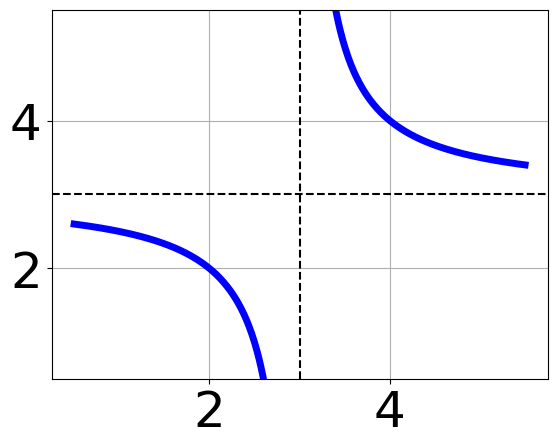
\includegraphics[width = 0.3\textwidth]{../Figures/rationalEquationToGraphBB.png}\item 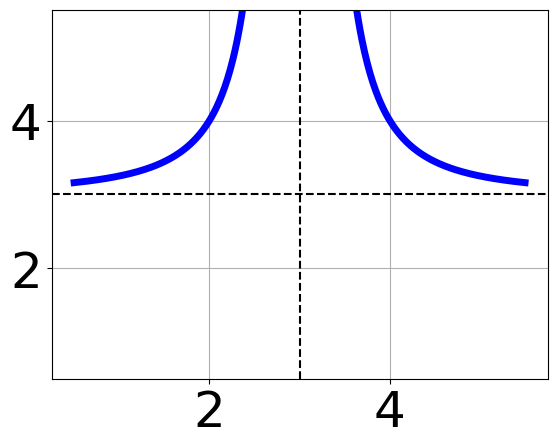
\includegraphics[width = 0.3\textwidth]{../Figures/rationalEquationToGraphCB.png}\item 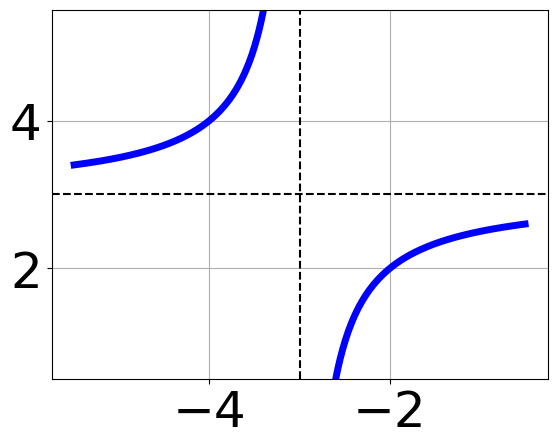
\includegraphics[width = 0.3\textwidth]{../Figures/rationalEquationToGraphDB.png}\end{multicols}\item None of the above.
\end{enumerate} }
\litem{
Choose the equation of the function graphed below.
\begin{center}
    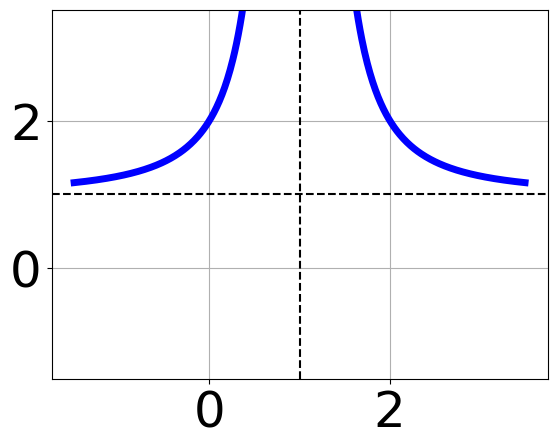
\includegraphics[width=0.5\textwidth]{../Figures/rationalGraphToEquationCopyB.png}
\end{center}
\begin{enumerate}[label=\Alph*.]
\item \( f(x) = \frac{-1}{x - 1} + 1 \)
\item \( f(x) = \frac{-1}{(x - 1)^2} + 1 \)
\item \( f(x) = \frac{1}{x + 1} + 1 \)
\item \( f(x) = \frac{1}{(x + 1)^2} + 1 \)
\item \( \text{None of the above} \)

\end{enumerate} }
\litem{
Choose the graph of the equation below.\[ f(x) = \frac{1}{(x + 1)^2} + 1 \]\begin{enumerate}[label=\Alph*.]
\begin{multicols}{2}\item 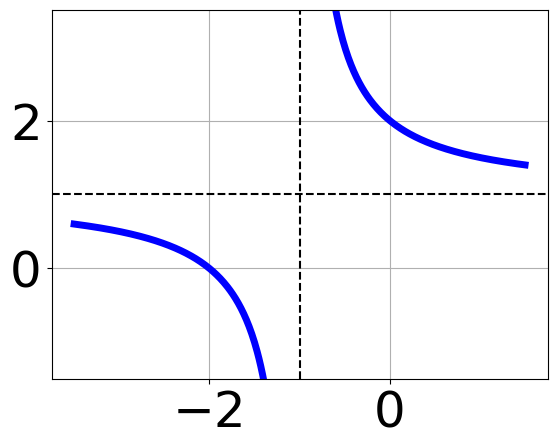
\includegraphics[width = 0.3\textwidth]{../Figures/rationalEquationToGraphCopyAB.png}\item 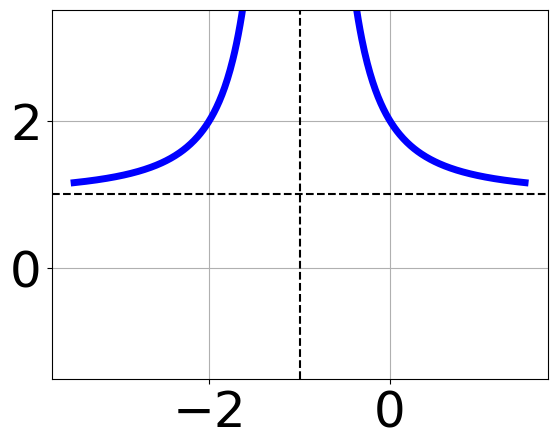
\includegraphics[width = 0.3\textwidth]{../Figures/rationalEquationToGraphCopyBB.png}\item 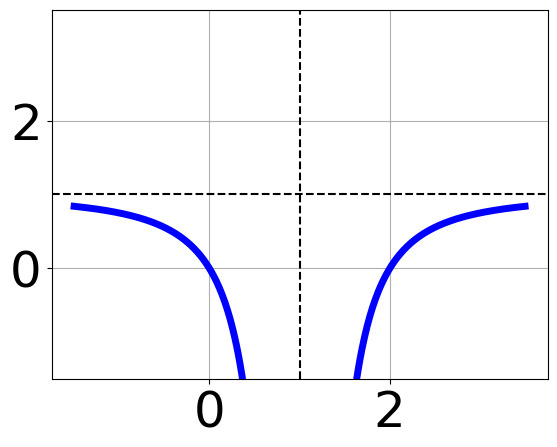
\includegraphics[width = 0.3\textwidth]{../Figures/rationalEquationToGraphCopyCB.png}\item 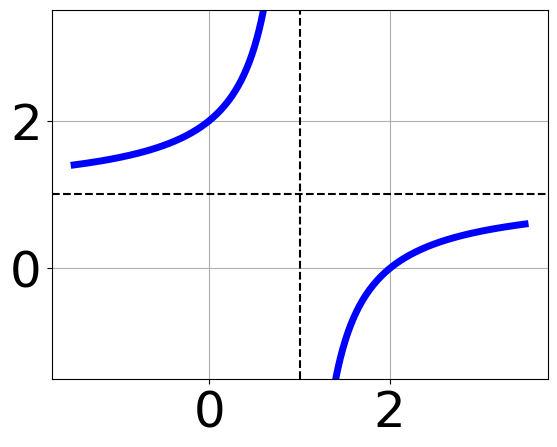
\includegraphics[width = 0.3\textwidth]{../Figures/rationalEquationToGraphCopyDB.png}\end{multicols}\item None of the above.
\end{enumerate} }
\litem{
Solve the rational equation below. Then, choose the interval(s) that the solution(s) belongs to.\[ \frac{126}{126x + 28} + 1 = \frac{126}{126x + 28} \]\begin{enumerate}[label=\Alph*.]
\item \( x \in [-0.22,0.78] \)
\item \( x \in [0,0.35] \)
\item \( x_1 \in [-0.43, 0.1] \text{ and } x_2 \in [0.17,0.33] \)
\item \( \text{All solutions lead to invalid or complex values in the equation.} \)
\item \( x_1 \in [-0.43, 0.1] \text{ and } x_2 \in [-0.28,-0.06] \)

\end{enumerate} }
\litem{
Solve the rational equation below. Then, choose the interval(s) that the solution(s) belongs to.\[ \frac{-7x}{5x -7} + \frac{-2x^{2}}{-15x^{2} +56 x -49} = \frac{6}{-3x + 7} \]\begin{enumerate}[label=\Alph*.]
\item \( x_1 \in [0.28, 0.85] \text{ and } x_2 \in [1.53,5.53] \)
\item \( \text{All solutions lead to invalid or complex values in the equation.} \)
\item \( x_1 \in [0.28, 0.85] \text{ and } x_2 \in [-0.6,2.4] \)
\item \( x \in [2.72,4.2] \)
\item \( x \in [1.99,3.46] \)

\end{enumerate} }
\litem{
Solve the rational equation below. Then, choose the interval(s) that the solution(s) belongs to.\[ \frac{-7}{5x -4} + 7 = \frac{6}{-10x + 8} \]\begin{enumerate}[label=\Alph*.]
\item \( \text{All solutions lead to invalid or complex values in the equation.} \)
\item \( x_1 \in [0.91, 4.91] \text{ and } x_2 \in [0.92,1.53] \)
\item \( x_1 \in [-2.69, 0.31] \text{ and } x_2 \in [0.8,1.16] \)
\item \( x \in [0.91,1.91] \)
\item \( x \in [-2.69,0.31] \)

\end{enumerate} }
\end{enumerate}

\end{document}